\section{Refracting Telescopes}

\makelabheader

{\bf Part 1: Theory}

Suppose that you have a telescope made of two lenses.  The ``objective''
lens has a focal length of 10 centimeters, and the ``eyepiece'' lens
has a focal length of 1 centimeter.  A refracting telescope is constructed
so that the two lenses are separated from each other by a distance
equal to the sum of their focal lengths (11 cm in this case).  That
way, one of the focal points of the objective matches up with one
of the focal points of the eyepiece
The setup is something like this:

\medskip

%\centerline{\epsfbox{figs/telescopefig1.eps}}
\centerline{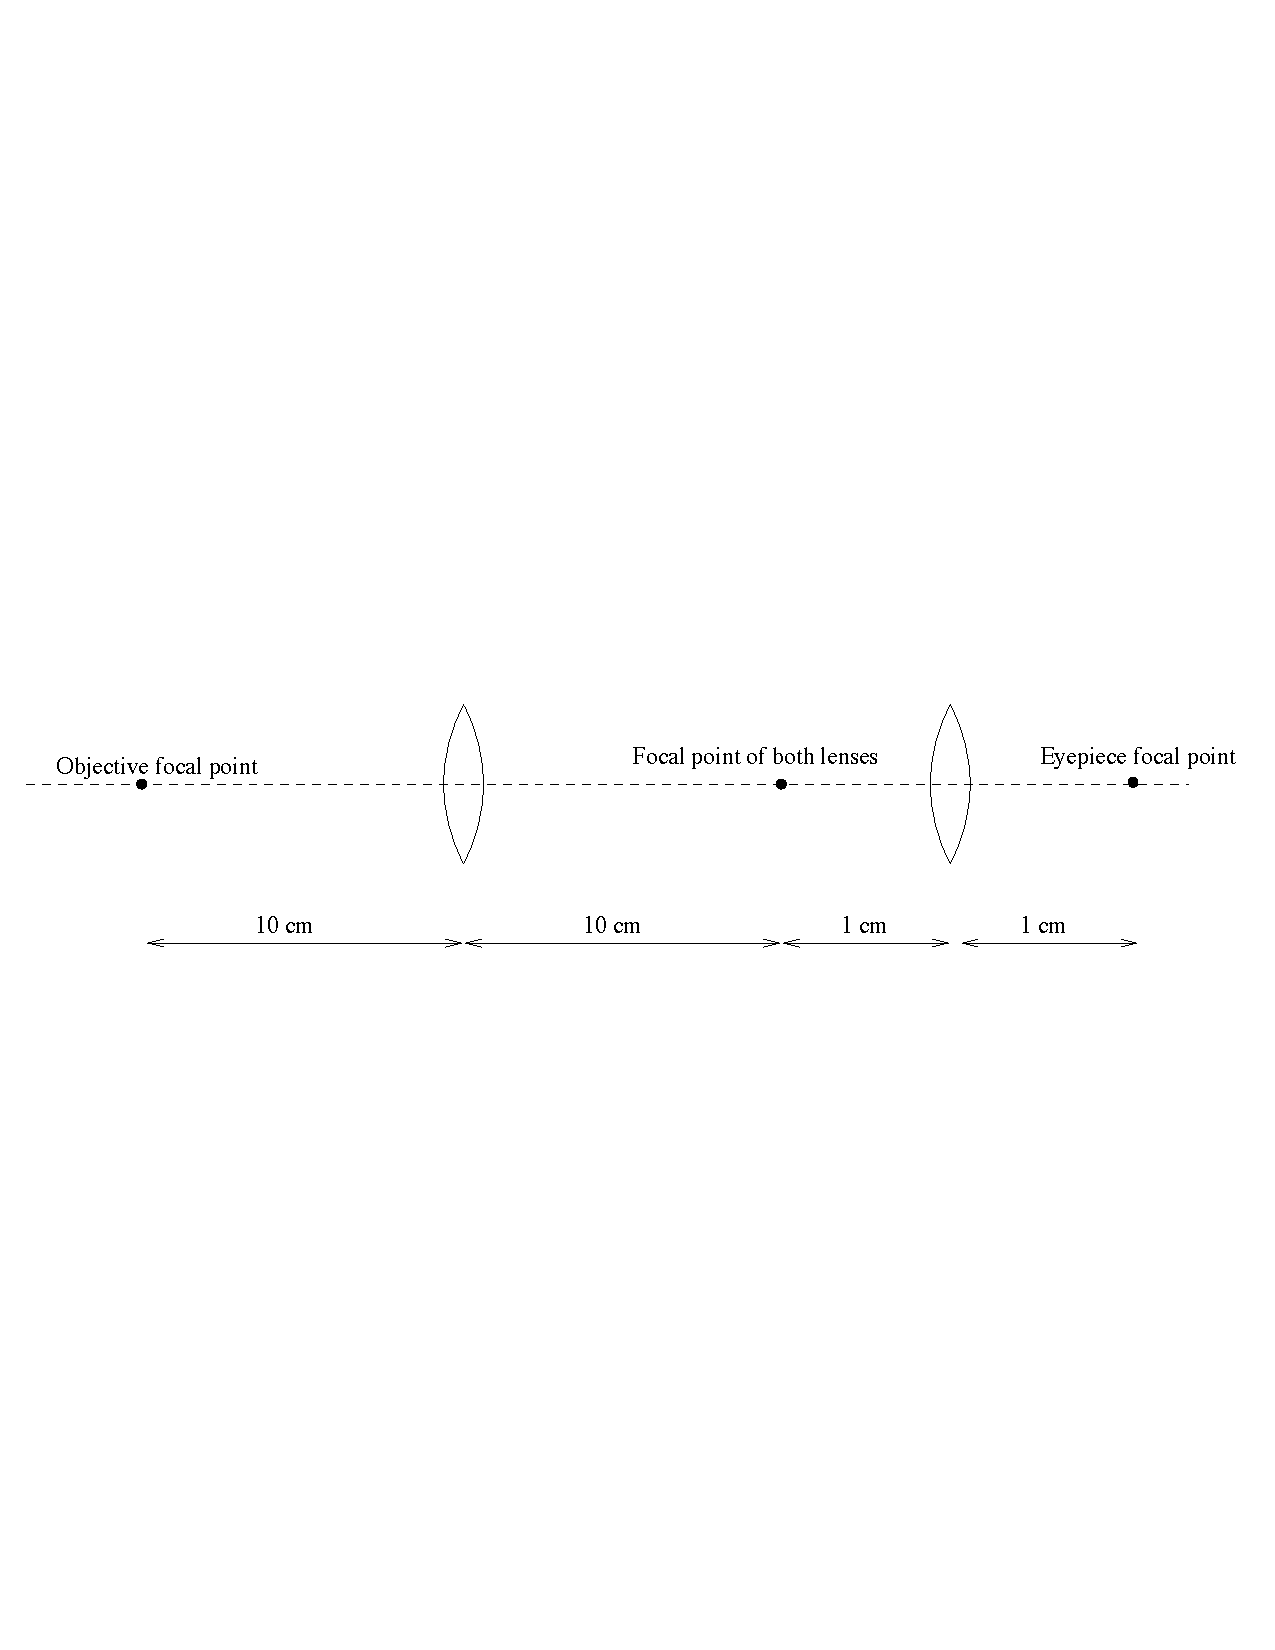
\includegraphics[width=\textwidth]{telescope/telescopefig1.pdf}}

\medskip

(Note that this picture is not to scale.)  The objective lens is on the
left, and the eyepiece is on the right.  The observer looks through
the eyepiece (not surprisingly) at a faraway object off to the left.

Suppose that you are using this telescope to look at an object that is
100 meters ($10^4$ centimeters) away.  We will work out where the
image of this object is produced, and how much it appears to be magnified.

The key facts that we'll need to do this are the rules you checked
in your last lab.  First, there's the relationship between the object 
position, the image position, and the focal length:
\begin{equation}
\frac{1}{p} + \frac{1}{q} = \frac{1}{f}.
\end{equation}
Second, there's the rule for the {\it linear magnification} of an image:
$$
\frac{h_i}{h_o}=\frac{q}{p}.
$$
Here $h_i$ is the height of the image produced by the telescope,
and $h_o$ is the height of the actual object.  The ratio of these two
is called the linear magnification $M$, so we'll write simply
\begin{equation}
M=\frac{q}{p}.  
\end{equation}
[Note: Often, the expression for the magnification is written with a minus sign
in it: $M=-{\frac{q} p}$.  It doesn't really matter for our purposes, though.]

In the calculations you're about to do, you'll be using known values of $p$ 
and $f$ and trying to find $q$.  So to make life simpler, take equation
(1) and solve it for $q$ in terms of $f$ and $p$.  (That is, rearrange
it so that it says $q=\ldots$.)  If you simplify this expression
as much as you can, you'll be less likely to make mistakes later.
(A good strategy is to isolate ${\frac{1} q}$ on one side of the equation,
then put the stuff on the other side over a common denominator, and
finally take the reciprocal.)  If you're not sure whether you've
got the right expression, show it to me.

\answerspace{2in}

Now suppose we have an object that is 100 m to the left of the telescope
above (so $p= 10^4$ cm).  The light passes through the objective lens
and forms an image (ignore the eyepiece for now).  Where is this
image?  Specifically, how far is it from the objective lens?  Also,
is it a real image or a virtual image?  When figuring out the
location of the image, record an answer in centimeters with at least
three digits after the decimal point.  (In other words, record
your answer to an accuracy of 0.001 cm.)

\answerspace{1in}

Mark the approximate location of this image with an $X$ on the diagram
above.
How far is this image from the eyepiece lens?  Again, record your answer
to an accuracy of 0.001 cm.

\answerspace{1in}

Calculate the linear magnification of this image using equation (2).
This should be a number between 0 and 1.  It indicates the factor
by which the image is smaller than the original object.

\answerspace{1in}


Now we want to figure out the effect of the eyepiece lens.  The big
idea here is that we treat the {\it image} produced by the objective
lens as if it were the {\it object} for the eyepiece lens.  That is,
we pretend that the image is a real thing that the eyepiece is examining.
That means that the answer to the previous question (distance
from the image to the eyepiece lens) becomes the new {\it object distance}
$p$.

Is the image produced by the eyepiece a real image or a virtual image?

\answerspace{1in}

How far away is the image produced by the eyepiece?
(When you calculate this, your answer for $q$ will come out negative.
That's OK: you can ignore the minus sign.  It just indicates that
the image is virtual.)

\answerspace{1in}

Now you know where the image will appear to be when you look through
the eyepiece.  Calculate the ratio of the distance to the original
object to the distance to the final image.  This is how many
times closer the telescope makes the object appear.

\answerspace{1in}

Use equation (1) to calculate the linear magnification of the image produced by 
the eyepiece.  This should be a number greater than 1.  It indicates
the factor by which the eyepiece has magnified the image.

\answerspace{1in}

The {\it overall linear magnification} of the telescope is the product
of the magnification produced by the objective lens and the magnification
produced by the eyepiece lens.  What is the overall 
linear magnification of this
telescope?

\answerspace{1in}

This number tells you how many times larger or smaller the final image
is than the original object.  
You should have found that this number is less than 1, which means
that the final image is actually {\it smaller} than the object.
That may seem surprising since we expect a telescope to make
things look bigger, not smaller.  What's going on here?

The point is that this linear magnification tells you how the
actual size of the image and object compare.  If you want to know
how big an object {\it looks}, you need to consider their
angular sizes.  The ratio of the angular size of the
final image to the angular size of the original object
is called the {\it angular magnification}.
What is the angular magnification of this telescope?

Hint: The angular size depends on both the actual size and the
distance.  You've already worked out what effect the telescope has on
the distance of the image (as compared to the object), and what effect
it has on the size of the image (as compared to the object).


\answerspace{1.5in}

There is a general rule that says that the angular magnification
of a telescope is equal to the ratio of the focal lengths $f_{\rm objective}/
f_{\rm eyepiece}$.  Is that true in this case?

\answerspace{1in}

{\bf Part 2: Constructing a Telescope}

In this part of the lab, you will use two lenses and some cardboard tubes
to construct a telescope.  

Determine the focal lengths of the two lenses, by any means you 
can think of.

\answerspace{1in}

According to the rule at the end of the last part, the angular
magnification of a telescope is the ratio of the focal lengths.
What is the angular magnification of a telescope constructed with
these lenses?

\answerspace{1in}

Insert the lenses into the tubes and adjust the distance between the lenses
until the telescope gives a sharply-focused image of faraway objects.

What is the orientation of an object as seen in the telescope?  Are
they upside-down?  Are they reversed left-to-right?

\answerspace{1in}

Stand in a location where you can see the eye chart posted on the wall.
Adjust your distance from the eye chart until you can just barely
read the F at the top of the chart (without using the telescope).
Now look at the chart with the telescope.  Which row is the
smallest row you can read using the telescope?  How many times
smaller is this row than the F at the top?  (The sizes of the letters
in each row are printed at the right of the chart.)
Compare this ratio with the angular magnification you calculated
for the telescope.  Do the results make sense?



